\documentclass{article}
\usepackage[utf8]{inputenc}
\usepackage[english]{babel}
\usepackage{amsmath}
\usepackage{amssymb}
\usepackage{setspace}
\usepackage{natbib} 
\usepackage{graphicx}
\usepackage{subfig}
\usepackage{comment}
\usepackage[backgroundcolor=pink,linecolor=red]{todonotes}
\usepackage{fullpage}
\usepackage[hidelinks]{hyperref}
\usepackage{xcolor}
\usepackage{comment}

\onehalfspacing


\title{Part 1 Demultiplexing | BIO 622}
\author{Jared Galloway}
\date{}                                           % Activate to display a given date or no date

\begin{document}
\maketitle

\section*{Part 1}

%\newpage
\begin{enumerate}
 \item 

\begin{center}
 \begin{tabular}{||c c||} 
 \hline
 Filename & Read \\ [0.5ex] 
 \hline\hline
 $1294_S1_L008_R1_001.fastq.gz$ & Read 1 \\ 
 \hline
 $1294_S1_L008_R2_001.fastq.gz$ & Index 1 \\
 \hline
 $1294_S1_L008_R3_001.fastq.gz$ & Index 2 \\
 \hline
 $1294_S1_L008_R4_001.fastq.gz$ & Read 2 \\
 \hline
\end{tabular}
\end{center}

 \item

\begin{description}

 \item

\begin{figure}[h!!!!]
	\center{
	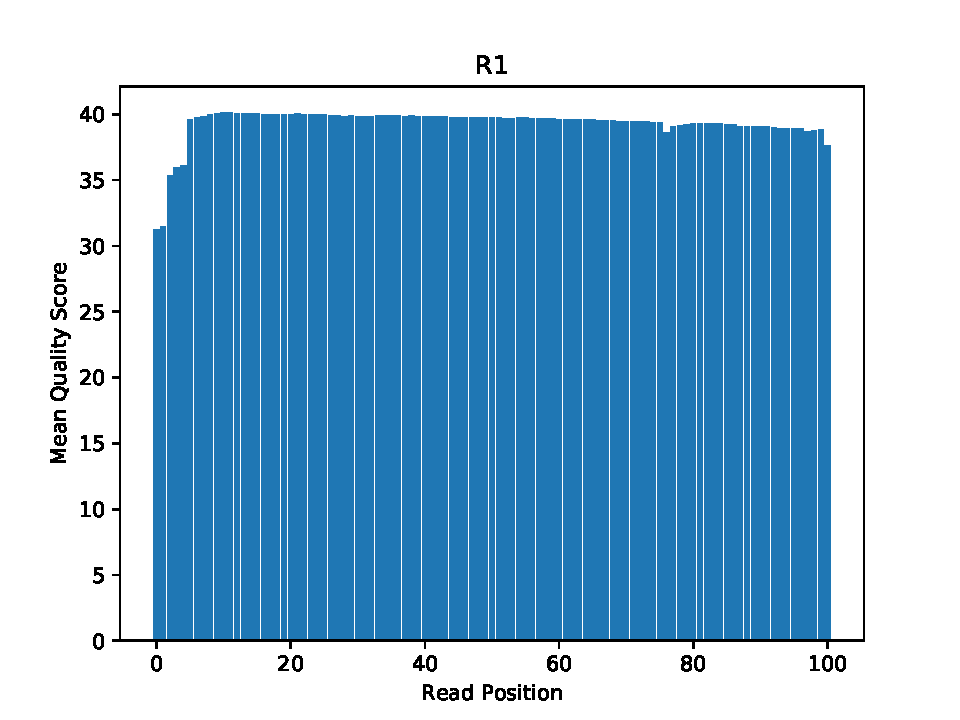
\includegraphics[width=0.8\textwidth]{../pos_dist_plots/tsv_hist1.pdf}
	}
	\caption{
	\label{fig:my-label1} Distribution of average quality score R1}
\end{figure}

\begin{figure}[h!!!!]
	\center{
	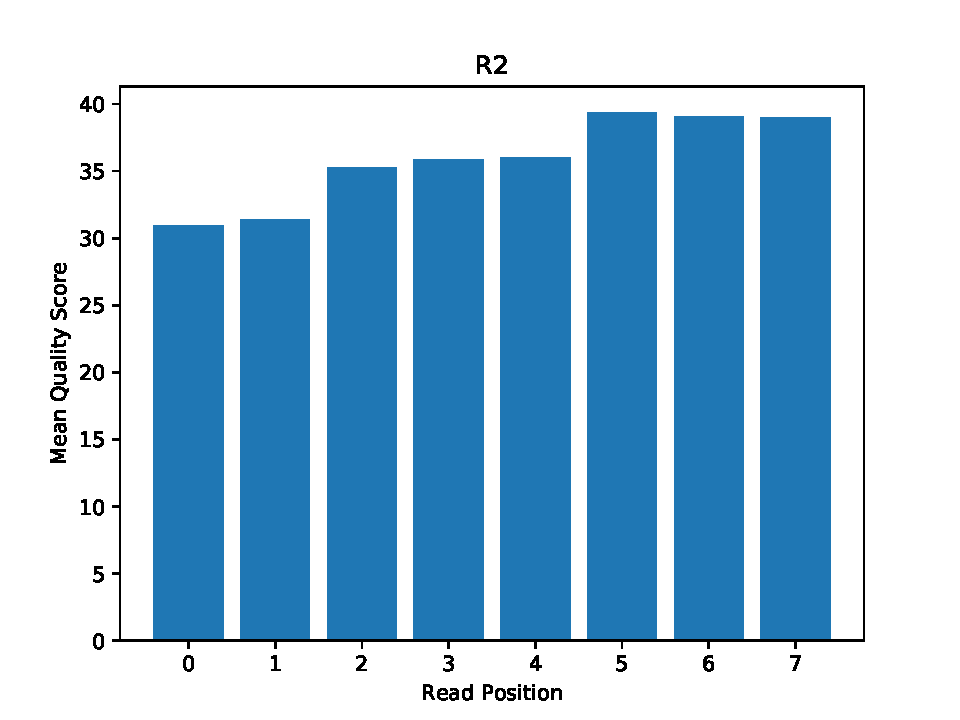
\includegraphics[width=0.8\textwidth]{../pos_dist_plots/tsv_hist2.pdf}
	}
	\caption{
	\label{fig:my-label}  Distribution of average quality score R2 }
\end{figure}

\begin{figure}[h!!!!]
	\center{
	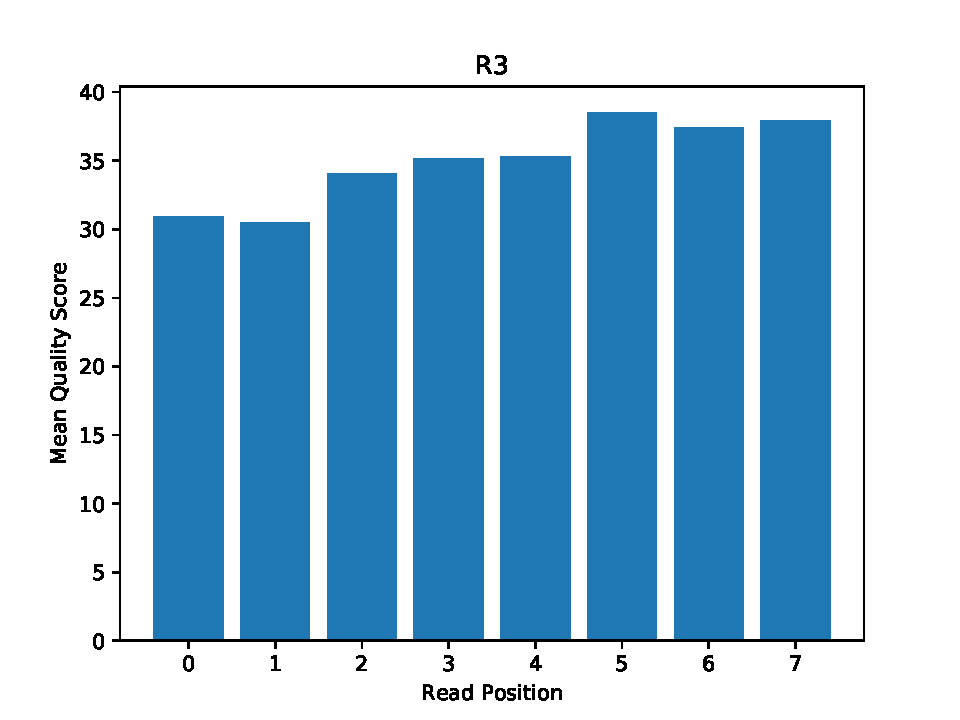
\includegraphics[width=0.8\textwidth]{../pos_dist_plots/tsv_hist3.pdf}
	}
	\caption{
	\label{fig:my-label}  Distribution of average quality score R3}
\end{figure}

\begin{figure}[h!!!!]
	\center{
	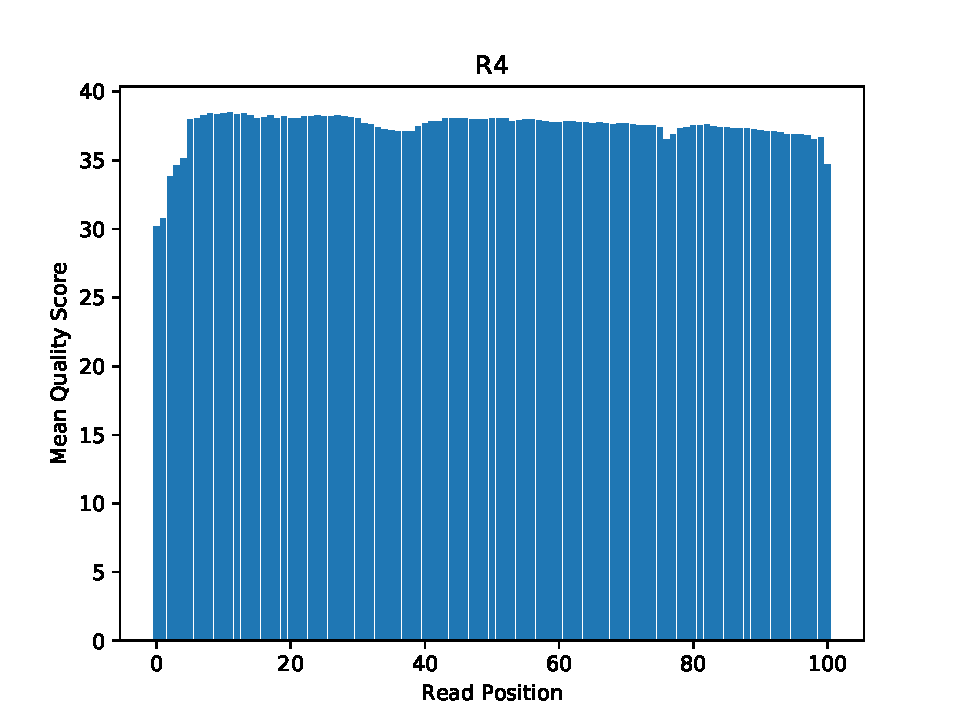
\includegraphics[width=0.8\textwidth]{../pos_dist_plots/tsv_hist4.pdf}
	}
	\caption{
	\label{fig:my-label}  Distribution of average quality score R4}
\end{figure}

\newpage
 \item

Due to the first two biologcal reads -- for both R1 and R2 -- 
are quite low $\approx < 36$, I would set the cutoff for 37, to make 
sure we are getting high quality biolocial reads.

\item

To find the total number of N's within the two index reads, 
I used the following bash command

\begin{center}

zcat emp\_files/1294\_S1\_L008\_R[2-3]* | awk 'NR\%4==2' | grep N | wc -l > countN_Index.txt

\end{center}

\begin{description}
\end{enumerate}
\end{document}
